% !TEX root = ../main.tex

\subsection{Implementation}
In this project we decided to implement a chorus effect by modulating the input signal with a varying delay. After modulation the original and modified signal are summed together. A visual presentation of the process is shown in \cref{fig:chorus}. Meanwhile we will only use one modulation channel in the implementation.


\begin{figure}[H]
	\centering
	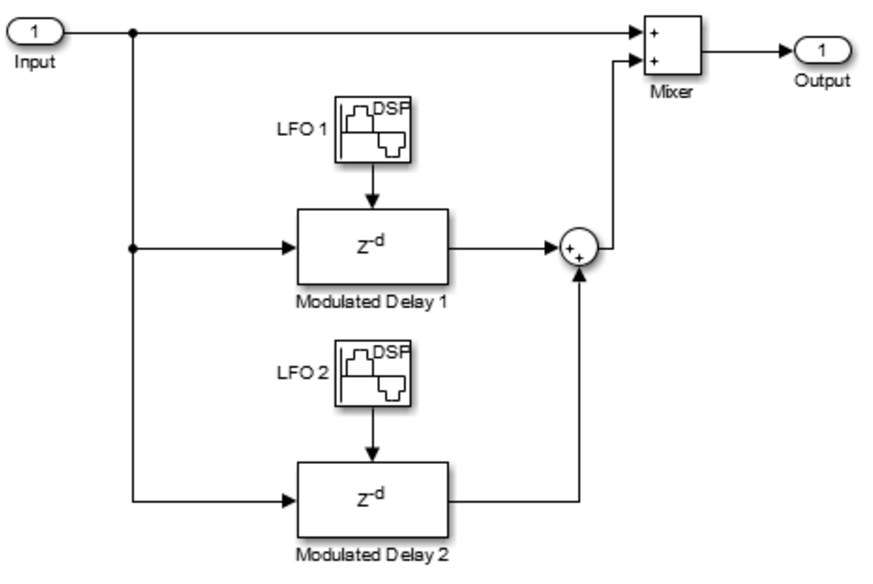
\includegraphics[width=0.5\textwidth]{modulation.png}
	\caption{Visual representation of the chorus modulation.}
	\label{fig:chorus}
\end{figure}

The resulting code for a chorus matlab script:

\begin{listing}[H]
	\begin{minted}[linenos,breaklines,stepnumber=5,frame=single]{matlab}
 %Import audio
 [x,Fs] = audioread('LeChuck_Theme.mp3'); 
 
 % Defining max delay in seconds
 max_time_delay=0.003;
 
 %Frequency of LFO
 rate=2;   
 
 % Sin reference to create oscillating delay
 index=1:length(x);
 sin_ref = (sin(2*pi*index*(rate/Fs)))';
 
 %Convert time delay to max delay in samples
 max_samp_delay=round(max_time_delay*Fs);
 
 % Create empty out vector
 y = zeros(length(x),1);
 
 % Set gain coefficient
 amp=0.7;
 
 % For each sample
 for i = (max_samp_delay+1):length(x),
 
 %Abs of current sin val 0-1
 cur_sin=abs(sin_ref(i)); 
 
 %Generate a varying delay  
 cur_delay=ceil(cur_sin*max_samp_delay);
 
 % Add delayed sample
 y(i) = (amp*x(i)) + amp*(x(i-cur_delay));
 end
 
	\end{minted}
	\caption{Matlab script for experimenting with the chorus effect.}
	\label{lst:chorus}
\end{listing}
